\chapter{机器人抓取规划实验结果及分析}
\label{ch:experiments}

本章通过仿真和真实抓取实验验证所提规划方法。实验分为两部分：首先比较不同方法生成抓取构型的分布特性；随后在真实机器人平台上统计抓取成功率。最后讨论方法的适用范围与局限性。

\section{实验环境及配置}
\label{sec:exp_setup}

\subsection{真实环境}
真实实验平台由 ABB GOFA-5 机械臂与 DH-ROBOTICS PGC 平行夹爪组成。夹爪最大行程为 76 mm，通过更换手指可分别配置为 0 到 76 mm 或 30 到 106 mm 两种开口范围；指腹为直径 28 mm、厚度 3 mm 的圆形垫片，摩擦系数约为 0.25。

实验共使用 9 个物体，包含开源数据集模型、工业件与日用品，并加入人工设计的四面体以测试极端几何场景。样本选择原因见附录 IV。

\begin{figure}[htbp]
    \centering
    % 请替换为实际图片文件名
    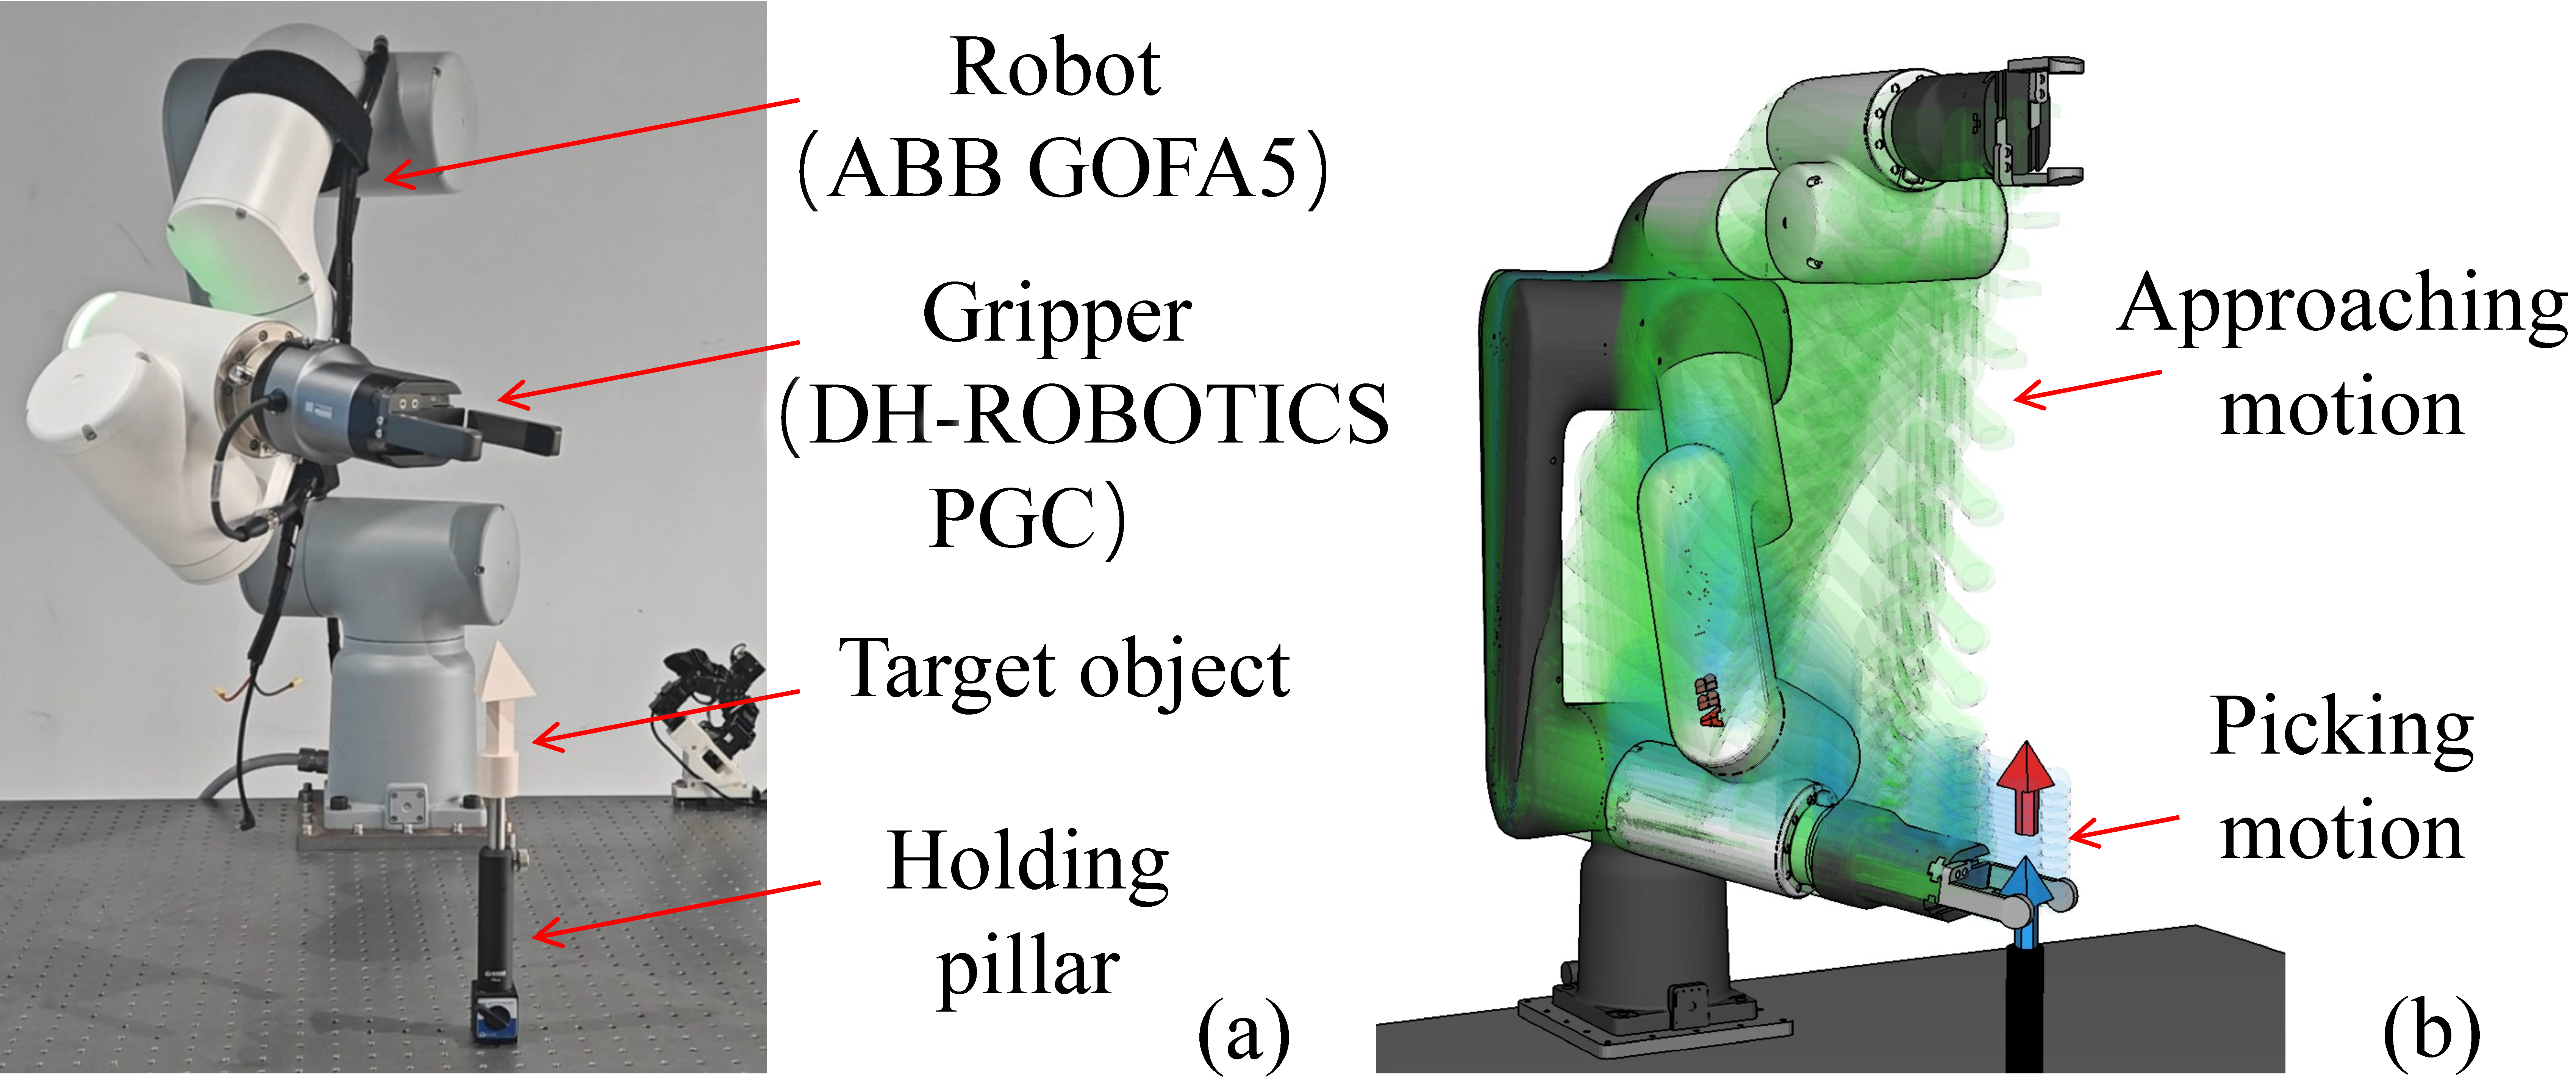
\includegraphics[width=0.8\linewidth]{FBGrasp/setting.pdf}
    \caption{(a) 真实物理实验场景设置；(b) 机器人运动规划路径示意：接近物体（绿色）、执行抓取（蓝色）及移动至目标位（绿色）。}
    \label{fig:setting}
\end{figure}

\subsection{仿真环境}
仿真实验用于定量分析抓取分布。为保证公平性，实验中物体位姿设为已知真值，不引入视觉误差。对比方法包括 GraspIt!、GPD 与 WRS，三者均在相同计算条件下运行。

\section{抓取分布多样性对比}
\label{sec:distribution_comparison}

\subsection{抓取分布统计指标}
除稳定性与可抓取性外，本文将抓取构型分布作为重要评价标准。分布越广、越均匀，机器人在复杂环境中的接近与执行灵活性越高。

具体地，统计对象为抓取构型的 6D 数据，并重点分析接触向量 $\mathbf{v}_i$。采用三个指标：标准差（STD）、极差（R）与平均绝对偏差（MAD）。为消除候选数量差异，每种方法均先生成超过 20 个候选，再统一降采样为 20 个。定量比较对象为四面体、Amicelli 和 Seal。

% 添加表格：分布指标对比
\begin{table}[htbp]
    \centering
    \small
    \setlength{\tabcolsep}{5pt}
    \caption{不同抓取规划方法在三个测试物体上的分布统计指标对比}
    \label{tab:distribution_metrics}
    \begin{threeparttable}
    \begin{tabular}{lcccc}
        \toprule
        \textbf{物体} & \textbf{方法} & \textbf{STD ($\uparrow$)} & \textbf{R ($\uparrow$)} & \textbf{MAD ($\uparrow$)} \\
        \midrule
        \multirow{4}{*}{四面体} 
        & GraspIt!~\cite{miller_graspit_2021} & 0.2516 & 0.8676 & 0.1998 \\
        & GPD~\cite{ten2017grasp} & 0.2878 & 0.9375 & 0.2389 \\
        & WRS~\cite{wan2020planning} & / & / & / \\
        & \textbf{本文方法} & \textbf{0.2995} & \textbf{0.9498} & \textbf{0.2450} \\
        \midrule
        \multirow{4}{*}{巧克力（Amicelli）} 
        & GraspIt!~\cite{miller_graspit_2021} & 0.1669 & 0.6687 & 0.1177 \\
        & GPD~\cite{ten2017grasp} & 0.2742 & 0.9454 & 0.2162 \\
        & WRS~\cite{wan2020planning} & 0.2639 & 0.9365 & 0.2002 \\
        & \textbf{本文方法} & \textbf{0.2835} & \textbf{0.9922} & \textbf{0.2193} \\
        \midrule
        \multirow{4}{*}{海豹（Seal）}
        & GraspIt!~\cite{miller_graspit_2021} & 0.2718 & 0.9063 & 0.2154 \\
        & GPD~\cite{ten2017grasp} & 0.2667 & 0.8409 & 0.2284 \\
        & WRS~\cite{wan2020planning} & 0.2427 & 0.8690 & 0.2014 \\
        & \textbf{本文方法} & \textbf{0.2857} & \textbf{0.9154} & \textbf{0.2429} \\
        \bottomrule
    \end{tabular}
    \begin{tablenotes}
        \footnotesize
        \item STD：标准差；R：极差；MAD：平均绝对偏差。
        \item WRS 对四面体无法生成有效抓取候选，以"/"表示。
    \end{tablenotes}
    \end{threeparttable}
\end{table}

\subsection{抓取分布可视化}
表 \ref{tab:distribution_metrics} 显示，本文方法在三个对象上的 STD、R、MAD 均为最优，说明生成的候选抓取覆盖范围更大、方向更分散。

图 \ref{exp:distribution}(a) 的夹爪可视化也支持这一结论。与主要依赖面接触的方法相比，本文方法可利用边缘与角点接触，在四面体等几何受限物体上仍能生成可行且多样的抓取。图 \ref{exp:distribution}(b) 的三维散点图进一步表明，本文方法在姿态空间中覆盖更广且分布更均匀。

\begin{figure}[htbp]
    \centering
    % 请替换为实际图片文件名
    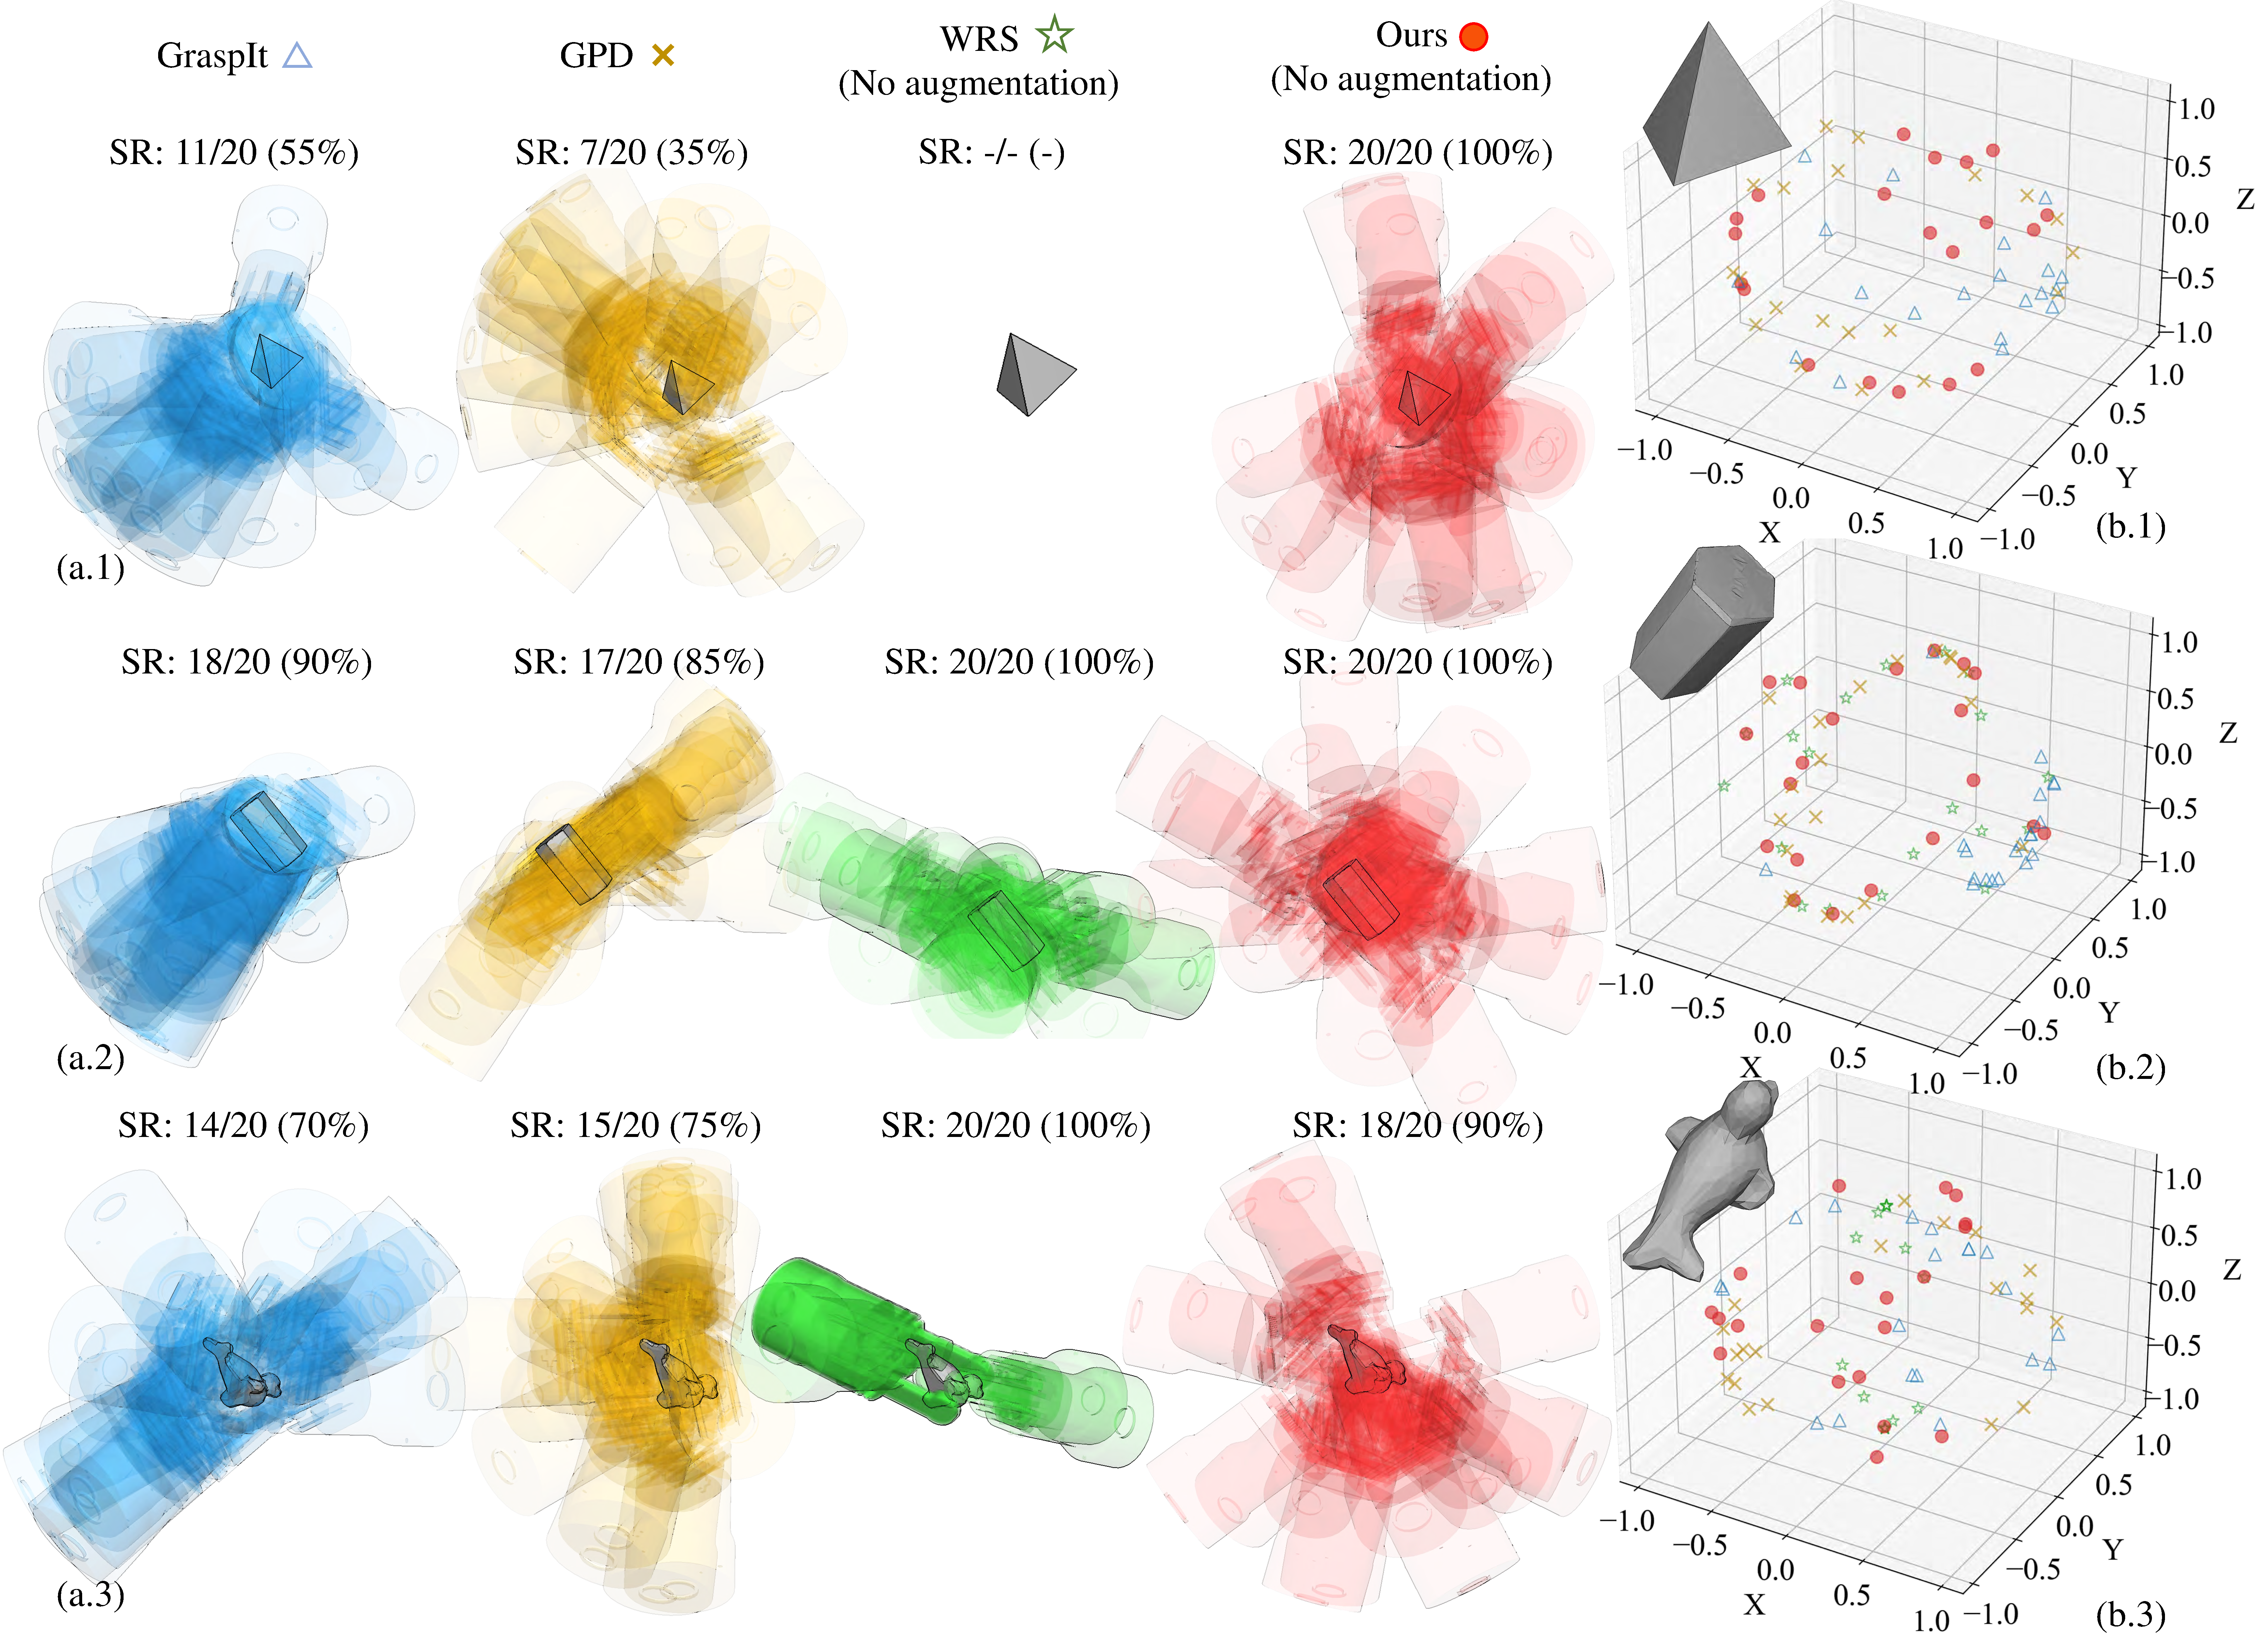
\includegraphics[width=1.0\linewidth]{FBGrasp/grasp_distribution_main.pdf}
    \caption{抓取分布可视化对比。(a) 各方法生成的抓取位姿展示（蓝色：GraspIt，黄色：GPD，绿色：WRS，红色：本文方法）；(b) 抓取构型在 3D 空间中的分布散点图。}
    \label{exp:distribution}
\end{figure}

\section{抓取成功率对比}
\label{sec:success_rate}

\subsection{实验设置与流程}
真实抓取实验在 ABB GOFA-5 平台上进行。为减少桌面碰撞并提升可达性，物体放置于细支撑柱上。运动规划采用 RRT-connect，任务流程为“接近、抓取、搬运到目标位”。为隔离视觉系统影响，实验中物体位姿均设为已知。

每个物体对每种方法执行 20 次抓取。若出现逆解不可达或碰撞，适当调整物体初始姿态以保证 20 个候选均可执行。成功标准为：物体被稳定提起并搬运，不发生滑落、脱落或明显姿态失稳。主要失败类型包括预接触碰撞、接触不足与构型不稳定。

\subsection{结果分析}
表 \ref{tab:statistical_results} 汇总了 9 个物体上的抓取成功率。本文方法平均成功率为 97.8\%，高于 WRS（76.7\%）、GPD（70.6\%）和 GraspIt（77.8\%）。

% 添加大表格：成功率对比
\begin{table*}[t]
    \centering
    \small
    \setlength{\tabcolsep}{4pt}
    \caption{各抓取规划方法的抓取成功率统计}
    \label{tab:statistical_results}
    \begin{threeparttable}
    \begin{tabular}{l|ccccccccc|c}
        \toprule
        \textbf{Method} & \textbf{四面体} & \textbf{巧克力} & \textbf{海豹} & \textbf{乐高} & \textbf{链轮} & \textbf{牛奶盒} & \textbf{杯面} & \textbf{电机座} & \textbf{齿轮} & \textbf{平均值} \\
        \midrule
        \textbf{Ours} & \textbf{100\%} & \textbf{100\%} & \textbf{90\%} & \textbf{100\%} & \textbf{100\%} & \textbf{95\%} & \textbf{95\%} & \textbf{100\%} & \textbf{100\%} & \textbf{97.8\%} \\
        WRS~\cite{wan2020planning} & 0\%   & 100\% & 100\% & 100\% & 95\%  & 95\% & 0\%  & 100\% & 100\% & 76.7\% \\
        GPD~\cite{ten2017grasp}& 35\%  & 85\%  & 75\%  & 85\%  & 85\%  & 70\% & 75\% & 70\%  & 55\%  & 70.6\% \\
        Graspit~\cite{miller_graspit_2021} & 55\%  & 90\%  & 70\%  & 90\%  & 80\%  & 80\% & 90\% & 75\%  & 70\%  & 77.8\% \\
        \bottomrule
    \end{tabular}
    \end{threeparttable}
\end{table*}

从单项结果看，WRS 在平行面物体上表现较好，但在四面体、杯面等缺少平行面的对象上无法生成有效抓取；GPD 与 GraspIt 可覆盖全部对象，但在锐边与复杂几何场景下成功率下降明显。本文方法对点、边、面接触统一建模，因此在四面体和齿轮等对象上仍保持较高成功率，体现了更好的几何适应性。

\section{本章小结}
\label{sec:summary}

本章通过分布统计与真实抓取测试验证了所提方法的有效性。仿真结果显示其抓取构型分布更广、更均匀；真实实验中平均成功率达到 97.8\%。

该方法目前仍是离线规划框架，依赖完整 3D 模型输入；同时主要面向平行夹爪，多指灵巧手场景仍需进一步扩展。尽管不同基线方法的参数调优机制不完全一致，实验结果仍能反映各方法在复杂几何接触条件下的能力差异。
